%coding:utf-8

%----------------------------------------
%FOSAPHY, a LaTeX-Code for a summary of linear systems and regulation
%Copyright (C) 2014, Mario Felder, Michael Fallegger

%This program is free software; you can redistribute it and/or
%modify it under the terms of the GNU General Public License
%as published by the Free Software Foundation; either version 2
%of the License, or (at your option) any later version.

%This program is distributed in the hope that it will be useful,
%but WITHOUT ANY WARRANTY; without even the implied warranty of
%MERCHANTABILITY or FITNESS FOR A PARTICULAR PURPOSE.  See the
%GNU General Public License for more details.
%----------------------------------------

\chapter{Teilsysteme}

\begin{center}
\begin{figure}[ht]
	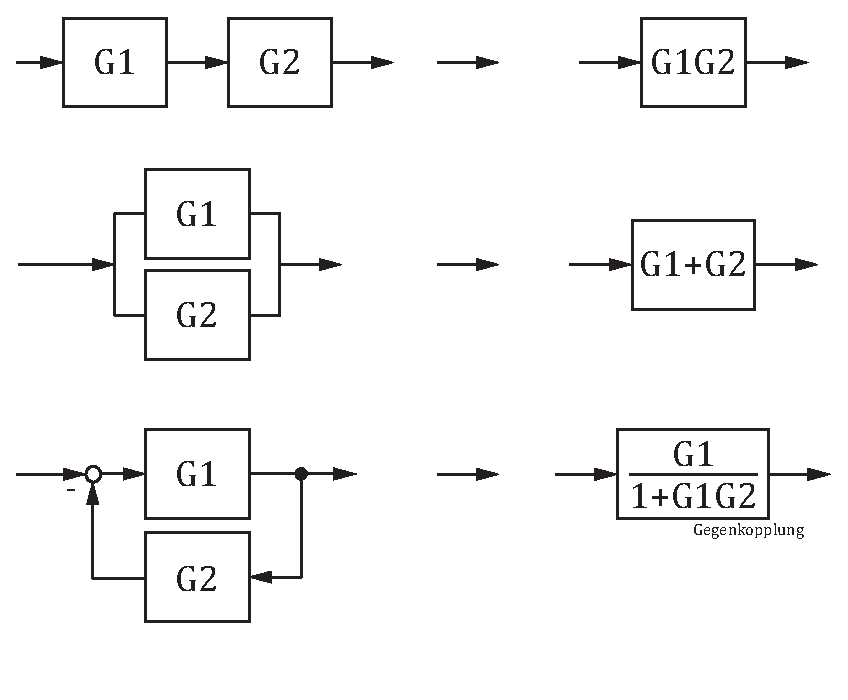
\includegraphics[scale = 0.62]{../fig/teilsysteme_p1.eps}
\end{figure}
\end{center}
\begin{center}
	\begin{figure}[ht]
	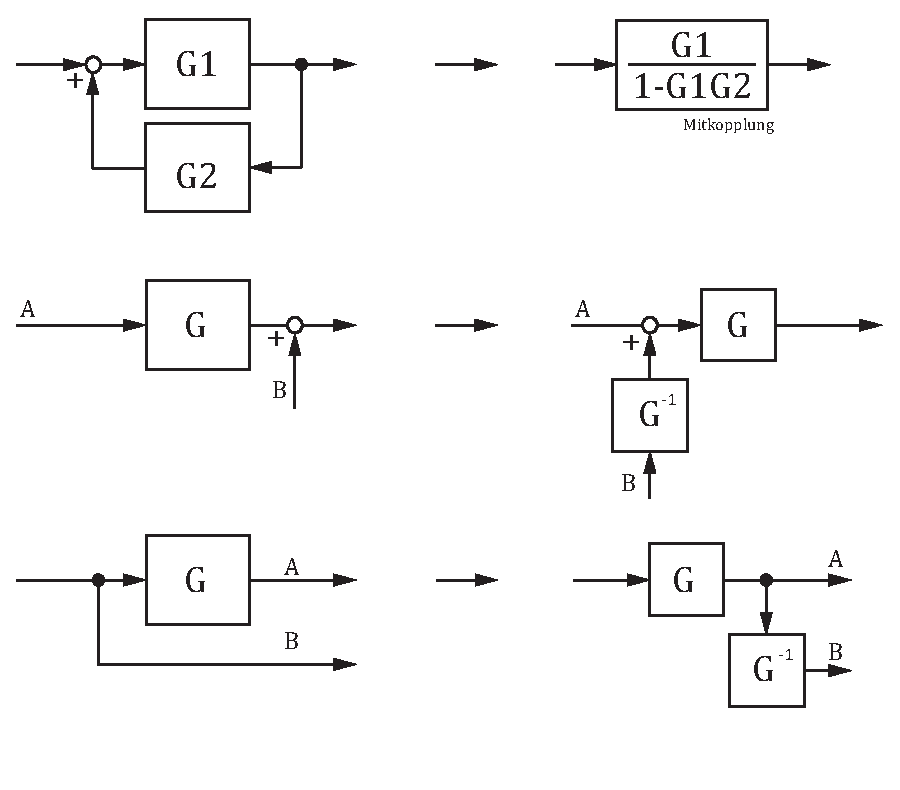
\includegraphics[scale = 0.62]{../fig/teilsysteme_p2.eps}
	\end{figure}
\end{center}
\
\\
\section{Flühlersche Regel}
Minuszeichen bei Summenpunkten können verschoben werden. Dadurch werden die Vorzeichen von nachfolgenden Summenpunkten invertiert.
\
Berechnungsprinzip:
\[
	G(s)=\frac{P_{V1}+P_{V2}+..}{1+P_{R1}+P_{R2}...}
\]
\begin{footnotesize}
	$P_V$:	Vorwärts laufende Pfade\\
	$P_R$:	Rückwärts laufende Pfade\\
\end{footnotesize}
